% !TEX root = replicas_draft.tex
\newcommand{\by}{\bar{y}}
\newcommand{\bw}{\bar{w}}
\newcommand{\bx}{\bar{x}}
\newcommand{\bu}{\bar{u}}
\newcommand{\bv}{\bar{v}}
\renewcommand{\ba}{\bar{a}}
\newcommand{\E}{{\cal E}}
\newcommand{\Hilbert}{{\rm H}}


\section{Single interval at finite temperature}

\la{sec:SingleInterval}

 We begin with the simple case of a single interval that contains one of the AdS$_2$ boundaries, as shown in figure 
 \ref{SingleIntervalSheets}(a). This is the interval $B \equiv  { [ 0, b ]}$.



To compute the entropy of this region we must consider the Euclidean path integral that evaluates the trace of powers of the density matrix $\Tr[\rho_B^n]$. This is given by the path integral on $n$ copies of the theory identified across the region $B$, as shown in figure \ref{SingleIntervalSheets}. The crucial point is that the presence of the branch point on the unit circle, which is where the asymptotic AdS boundary lives, elongates this circle by a factor of $n$. The Euclidean gravity configurations we must consider are all smooth manifolds with a single boundary that is identified with this elongated AdS boundary.

\begin{figure}
\begin{center}
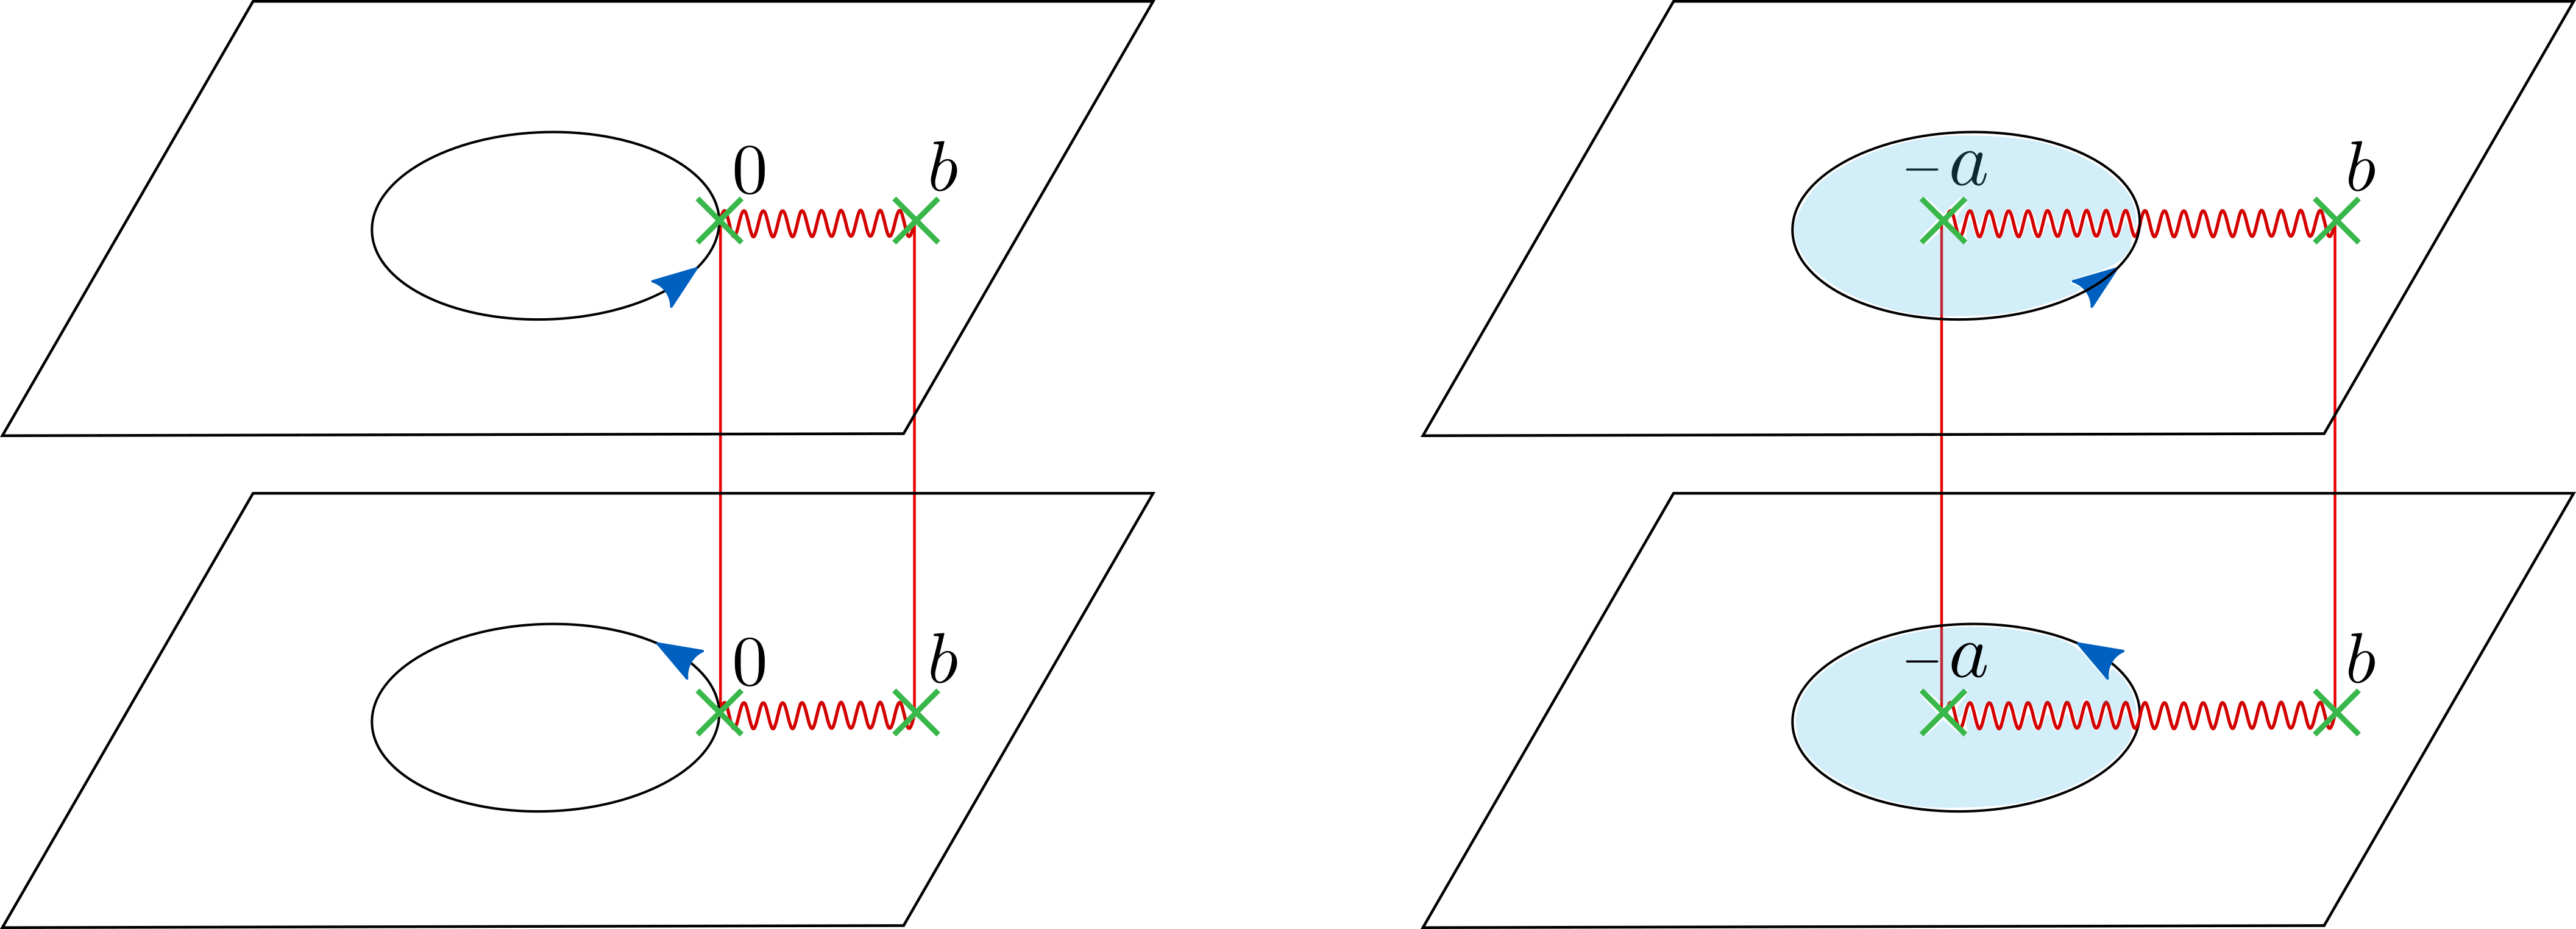
\includegraphics[scale=0.5]{figures/SingleIntervalSheets}

(a) ~~~~~~~~~~~~~~~~~~~~~~~~~~~~~~~~~~~~~~~~~~~~~~~~~~~~ ~~~~~(b)
\end{center}
\caption{\small  
(a) We have a flat space field theory on the exterior of the disk. The disk is hollow in this picture, and will be filled in with gravitational configurations subject to the boundary conditions on the unit circle. 
 This boundary is connected into a single long circle $n$ times longer than the original one. This is indicated by the blue arrow which tells you how to go around the cut. (b) The disk is filled in with a gravitational configuration with the topology of a disk which ends on the elongated unit circle.  This configuration can be represented by adding a branch point inside. Note that the local geometry at the branch point ``$-a$'' is completely smooth.  
\label{SingleIntervalSheets}}
\end{figure}

The simplest configuration to consider will be that with the topology of a disk. All other higher genus manifolds will be subleading since each extra handle will come with a cost of $e^{-S_0}$. Filling out the gravity region has the effect of extending the identification across the different sheets into the gravity region, which ends on some point ``$-a$'' in figure \ref{SingleIntervalSheets}. The location of the point ``$-a$'' will be dynamically determined by the saddle point of the path integral.


\begin{figure}
\begin{center}
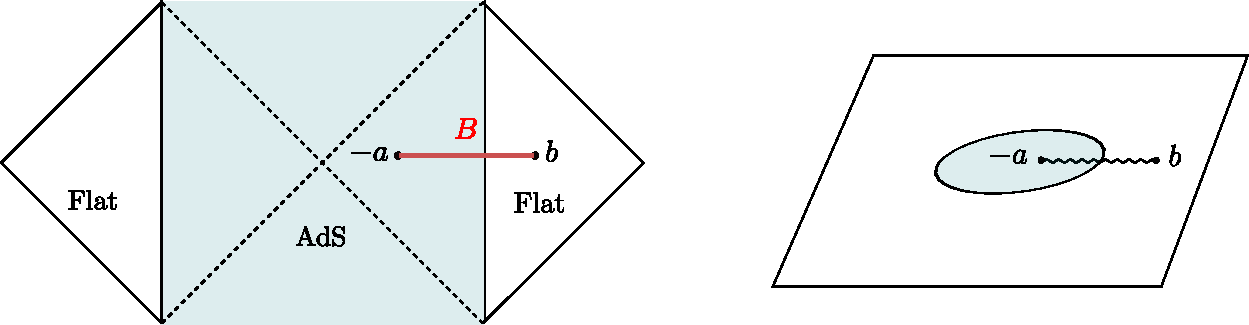
\includegraphics[scale=0.7]{figures/single-interval.pdf}
\end{center}
\caption{\small The single interval configuration in Lorentzian signature (left) and in Euclidean signature (right).  
\label{SingleLandE}}
\end{figure}

We will now construct replica wormholes explicitly for a single interval in the eternal black hole in AdS$_2$.  The Lorentzian and Euclidean geometries are shown in figure \ref{SingleLandE}. 
 We will first review of the result of the QES calculation \cite{Almheiri:2019yqk}, then proceed to derive it from replica wormholes.


\subsection{Geometry of the black hole}


The metric of eternal  black hole, glued to flat space on both sides, is
\be\label{dsyin}
ds^2_{\rm in} = \frac{4\pi^2}{\beta^2}\frac{dy d\by}{ \sinh^2 \frac{\pi}{\beta}(y+\by)} , \qquad
ds^2_{\rm out} = \frac{1}{\epsilon^2} dy d\by \ , 
\ee
\be
y = \sigma + i \tau ,\qquad \by = \sigma - i \tau  ~,~~~~~\tau = \tau + \beta  \ .
\ee
The subscript `in' refers to the gravity zone, and `out' refers to the matter zone\footnote{The Poincare coordinates are $ x = \tanh{ \pi y \over \beta } $, $ds^2_{\rm in} = 4 d x d\bar x/(x+\bar x)^2$. The  Schwarzschild coordinates are \be
y = \frac{\beta}{2\pi}\log \frac{r}{\sqrt{r(r + 4\pi/\beta)}}  + i \tau  \ ,  \qquad
ds^2_{in} = r(r + \frac{4\pi}{\beta})d\tau^2 + \frac{dr^2}{r(r + \frac{4\pi}{\beta})}  \ .
\ee   }. The interface is along the circle $\sigma = -\epsilon$. 
 Lorenztian time $t$ is  $\tau = -it$. 
The welding maps of figure \ref{WandZplanes} are trivial  and we have
\begin{align} \la{wexpy}
z=v= w = e^{2 \pi y /\beta} \ , \qquad y = \frac{\beta}{2\pi}{\log w} \ .
\end{align}
The Euclidean solution is   therefore the $w$-plane with gravity inside the unit disk, $|w|  <  1 - \frac{2\pi \epsilon}{\beta}$. The metric is
\be\label{xmet}
ds^2_{\rm in} =  \frac{4dw d\bw}{(1-|w|^2)^2} , \qquad   \qquad 
ds^2_{\rm out} =\frac{\beta^2}{4\pi^2\epsilon^2} \frac{dw d\bw}{|w|^2} \ .
\ee
The dilaton, which is defined only on the inside region, is rotationally invariant on the $w$-plane, 
\be \la{DilExpr}
\phi = \frac{2\pi \phi_r}{\beta} \frac{1 + |w|^2}{1 - |w|^2} = -{ 2 \pi \phi_r \over \beta }{ 1 \over \tanh{ 2\pi \sigma \over \beta } }   \ .
\ee
 with $\phi = \phi_r/\epsilon$ at the boundary. In what follows, we will usually set $\epsilon = 0$, and rescale the exterior coordinate by $\epsilon$ so that $ds^2_{out} = dy d\by$. 

\subsection{Quantum extremal surface}

We now review the computation of the entropy of the region $B = { [0,b]}$ which includes the $AdS_2$ 
boundary, see figure \ref{SingleIntervalSheets}.  
In gravity this will involve an interval $[-a,b]$, with  
 $a, b > 0$, see figure \ref{SingleLandE}. 


 
The generalized entropy of the region $[-a,b]$ is
\be \la{SgenGen}
S_{\rm gen} = S_0 + \phi(-a) +  
S_{\rm CFT}([-a,b]) \ .
\ee
The entanglement entropy of a CFT on the interval $[w_1,w_2]$ in the metric $ds^2=\Omega^{-2} dw d\bw$ is
\be\label{scftgeneral}
S_{\rm CFT}(w_1, w_2) = \frac{c}{6}\log \left(\frac{ |w_1 - w_2|^2 }{\epsilon_{1,UV} \epsilon_{2,UV} \Omega(w_1, \bw_1) \Omega(w_2, \bw_2) } \right) \ .
\ee
Using the map $w = e^{2 \pi y/\beta}$ and the conformal factors in \eqref{xmet} this becomes
\begin{align}
S_{\rm CFT}([-a,b]) &= 
 \frac{c}{6}\log \left(  \frac{2\beta\sinh^2 \left( \frac{\pi}{\beta} (a+b)\right) }{\epsilon_{a,UV} \epsilon_{b,UV} \pi    \sinh \left( \frac{2\pi a}{\beta} \right)}\right)
\end{align}
Then, using the dilaton in \nref{DilExpr}, \nref{SgenGen} becomes 
\begin{align}\label{sgens}
S_{\rm gen}([-a,b]) &=
S_0 + \frac{2\pi \phi_r}{\beta}\frac{1}{\tanh \left( \frac{2\pi a}{\beta} \right)  } 
+   \frac{c}{6}\log \left( \frac{2\beta\sinh^2\left( \frac{\pi}{\beta}(a+b) \right) }{ \pi \epsilon \sinh \left( \frac{2 \pi a}{\beta}\right)} \right) \ .
\end{align}
The UV divergence $\epsilon_{a,UV}$ was absorbed into $S_0$ and we dropped the outside one at point $b$. 
The quantum extremal surface is defined by extremizing $S_{\rm gen}$ over $a$ 
\begin{align} \label{tzeroex2}
\partial_a S_{\rm gen} =0 ~~\to~~~~~~ \sinh \left(\frac{2\pi a}{\beta} \right) =  \frac{12 \pi \phi_r}{\beta c} \frac{\sinh \left( \frac{\pi}{\beta}(b+a)\right)}{\sinh \left( \frac{\pi}{\beta}(a-b)\right)}
\end{align}
This is a cubic equation for $e^{2\pi a/\beta}$. For $b \gtrsim \frac{\beta}{2\pi}$  and $\phi_r/(\beta c) \gtrsim 1$,  the solution is
\be \la{smallAB}
a \approx b  + \frac{\beta}{2\pi}\log \left( \frac{24 \pi \phi_r}{\beta c}\right) ~, ~~~~~~{\rm or } ~~~~~ e^{ - { 2\pi a \over \beta} }\approx  { \beta c \over 24 \pi \phi_r } { e^{-{ 2 \pi b \over \beta } } 
} 
\ee
Since we've restricted to one side of the black hole in this calculation, the configuration is invariant under translations in the Schwarzschild $t$ direction. Therefore the general extremal surface at $t\neq 0$ is related by a time translation; for an interval that starts at $t_b$ and $\sigma_b = b$, the other endpoint is at 
  $t_a = t_b$ and $\sigma_a=-a$, with $a$ as in   \eqref{tzeroex2}.


\subsection{Setting up the  replica geometries }

We will do the replica calculation in Euclidean signature, with $a,b$ real. We set $\beta = 2\pi$, and reintroduce it later by dimensional analysis. 

The replica wormhole that we seek is an $n$-fold cover of the Euclidean black hole, branched at the points $a$ and $b$, 
see figure \nref{SingleLandE}. 
This manifold will have a nontrivial gluing at the unit circle (unlike the black hole itself), so it is more convenient to introduce different coordinates on the inside and outside. We use $w$, with $|w| < 1$, for the inside and 
$v = e^y$, with $|v|>1$ for the outside.    The gluing function is $\theta(\tau)$, with 
$
w = e^{i \theta} $, $ v = e^{i\tau} $, as in \nref{WeldEqns}. 
We write the branch points as 
\be
w = A = e^{-a} \ , \qquad v = B = e^b \ .
\ee

The Schwarzian equation is simplest in a different coordinate, 
\be \la{wtildew}
\widetilde{w} = \left( \frac{w - A}{1 - A w} \right)^{1/n} \ .
\ee
This coordinate uniformizes $n$ copies of the unit disk, so here we have the standard hyperbolic metric,
\be \la{metrictil}
ds^2_{in} = \frac{4 |d\tilde{w}|^2}{(1 - |\tilde{w}|^2)^2} \ .
\ee
Defining   $\tilde w = e^{ i \tilde \theta}$ at the boundary, the Schwarzian equation is
\be\label{schwtilde}
\frac{\phi_r}{2\pi} \p_{\tau} \{e^{ i \tilde \theta}, \tau\} = i(T_{yy}(i\tau) - T_{\by\by}(-i\tau)) \ .
\ee
We can now return to the $w$-disk using the Schwarzian composition identity
\be
\{e^{ i \tilde \theta} , \tau\} = \{ e^{i \theta}, \tau\}  + \frac{1}{2}\left(1- \frac{1}{n^2} \right) R(\theta) \ , 
\ee
with
\be \la{Rdefi}
R(\theta) = - \frac{(1-A^2)^2 ( \partial_\tau \theta)^2 }{ |1  - Ae^{i\theta}|^4  } \ .
\ee
This puts the equation of motion \eqref{schwtilde} into exactly the form of equation  \eqref{EOMFin}, which we have just derived by a slightly different route. In appendix \ref{GravAct} we show that they are equivalent. 

The stress tensor appearing on the right-hand side of \eqref{schwtilde} is obtained through the conformal welding. That is, we define the $z$ coordinate by the map $G$ on the inside and $F$ on the outside as in \eqref{WeldEqns}. These maps each have an ambiguity under $SL(2,C)$ transformations of $z$, which we may use to map the twist operator at $w = A$ to $z=0$, and the twist operator at $v = B$ to $z = \infty$. We further discuss the symmetries of the conformal welding problem in appendix \ref{app:welding}.

The $z$-coordinate covers the full plane holomorphically. It has twist points at the origin and at infinity, which can be removed by the standard mapping, $\tilde{z} = z^{1/n}$. On the $\tilde{z}$ plane, the stress tensor vanishes, so on the $z$-plane,
\be
T_{zz}(z) = -\frac{c}{24\pi} \{ z^{1/n}, z \} = -\frac{c}{48\pi}\left(1 - \frac{1}{n^2}\right) \frac{1}{z^2} \ .
\ee
Finally the stress tensor $T_{yy}$ comes from inverting the conformal welding map to return to the $v$-plane, and using $v = e^{y}$:
\be
T_{yy}(y) = e^{2y}\left[ F'(v)^2 T_{zz} - \frac{c}{24\pi}\{ F, v \} \right]  - \half \ .
\ee
Putting it all together, the equation of motion \eqref{schwtilde} is
\be \label{singleintervalEOM}
\frac{24 \pi \phi_r  }{c \beta}\p_\tau
\left[ \{ e^{i\theta(\tau)}, \tau \} + \frac{1}{2} (1- \frac{1}{n^2} ) R(\theta(\tau)) \right] = 
ie^{2i\tau}\left[ 
 - \frac{1}{2}(1 - \frac{1}{n^2}) \frac{F'(e^{i\tau})^2}{F(e^{i\tau})^2} -  \{F, e^{i\tau} \} \right]  + cc
\ee
This equation originated on the smooth replica manifold $\widetilde{{\cal M}}_n$, but has now been written entirely on the quotient manifold ${\cal M}_{n} = \widetilde{{\cal M}}_n/\mathbf{Z}_n$.  We have restored the nontrivial temperature dependence\footnote{The trivial temperature dependence is restored by $\tau \to {  2 \pi \over \beta }\tau_{phys}$, with $\tau_{phys}$ the physical Euclidean time with period $\beta$.}. In particular, note that $\theta(\tau+ 2\pi) = \theta + 2 \pi$. The $\tau \rightarrow -\tau$ symmetry of the insertions allows us to choose a function $\theta(\tau) = - \theta(-\tau)$ which will automatically obey $\theta(0)=0$, $\theta''(0)=0$. In addition, we should then impose $\theta(\pi) = \pi$ and $\theta''(\pi) =0$. The problem now is such that $n$ appears as a continuous parameter and there is no difficulty in analytically continuing in $n$. 

This is our final answer for the equation of motion at finite $n$. It is quite complicated, because the welding map $F$ depends implicitly on the gluing function $\theta(\tau)$.  We will solve it in two limits: $\beta \to 0$ at any $n$, and $n \to 1$ at any $\beta$.



\subsection{Replica solution as $n \to 1$}

We will now show that the equation of motion \eqref{singleintervalEOM} reproduces the equation for the quantum extremal surface.


We start with the solution for $n=1$. In this case the welding problem is trivial and we can set $w =v $ everywhere. 
It is convenient to set 
\be \la{zChoice}
 z = F(v) = { v - A \over B - v} = G(w) ~,~~~~~w=v
 \ee
   At $n=1$ any choice of $A$ can do. Different choices of $A$ can be related by an 
 $SL(2,R)$ transformation that acts on $w$. It will be convenient for us to choose $A$ so that when we go to $n\sim 1$, it corresponds to the position of the conical singularity. 
 

 
We now go near $n \sim 1$ and expand
\be
e^{i\theta} = e^{i\tau} + 
e^{ i \tau} i \delta \theta(\tau) \ ,
\ee
where $\delta \theta$ is of order $n-1$. 
We aim to solve
 \eqref{singleintervalEOM} for $\delta \theta$. 
The first step is to find the welding map perturbatively in $(n-1)$. 
In appendix \ref{app:welding}, we show that
\be
e^{2i\tau} \{ F , e^{i \tau} \} = -\delta\{e^{i\theta} , \tau \}_-  = -(\delta \theta''' + \delta \theta' )_-
\ee
where we used
\be \delta \{ e^{i\theta} ,\tau \} \equiv \{ e^{ i \tau + i \delta \theta} , \tau \} - \{ e^{ i \tau } , \tau \} = \delta \theta''' + \delta \theta' 
\ee
The minus subscript indicates that this is projected onto negative-frequency modes. This can be written neatly using the Hilbert transform, $\Hilbert$, which is defined by the action $\Hilbert \cdot e^{i m \tau} = - \mbox{sgn} (m) e^{im \tau}$ (and $\Hilbert \cdot 1 = 0$). Then
\be \la{HilH}
e^{ 2 i \tau } \{ F , e^{i \tau} \} = -\half (1 +\Hilbert)
(\delta \theta''' + \delta \theta' )  .
\ee
Wherever else $F$ appears in \eqref{singleintervalEOM}, it is multiplied by $(n-1)$, so there we can set $F = \frac{v-A}{B-v}$, as in \nref{zChoice}. Therefore the equation of motion for the perturbation is
\be\label{hilbertp}
\p_\tau (\delta \theta''' + \delta \theta' ) + \frac{ic}{12 \phi_r} \Hilbert \cdot (\delta \theta''' + \delta \theta' ) = (n-1) \left[ \frac{c}{12\phi_r}{\cal F} -\p_\tau R(\tau) \right]
\ee
where 
\be\label{fluxdefFull}
{\cal F} = -i  \frac{e^{2 i \tau}  (A - B)^2}{ (e^{i \tau} - A )^2 (e^{ i \tau} - B)^2} + cc  \ .
\ee
Equation \eqref{hilbertp} is nonlocal, due to the Hilbert transform. 
We can solve it by expanding both sides in a Fourier series. 
The important observation is that, due to the structure of derivatives in each term of the left hand side of \nref{hilbertp},  the terms with 
Fourier modes of the form $e^{ik \tau}$ for $k = 0, \pm 1$ are automatically  zero in the left hand side. Therefore, in order to solve this equation, we must impose the same condition on the right-hand side. The $k =  1$ mode requires
\be
\int_{0}^{2\pi}d\tau e^{-i\tau} \left( \frac{c}{12\phi_r}{\cal F} -\p_\tau R(\tau) \right) = 0 \ .
\ee
Doing the integrals, this gives the condition
\be
\frac{c}{6 \phi_r} \frac{ \sinh \frac{a-b}{2} }{ \sinh \frac{b+a}{2} }  = \frac{1}{\sinh a } ~.~~~~~~    \ee
This matches the equation for the quantum extremal surface \eqref{tzeroex2} that came from the derivative of the generalized entropy.
The term with $k=0$ is automatically zero in the right hand side, as  $\partial_\tau R$ is explicitly a total derivative and   $ \int_0^{2\pi } d\tau {\cal F} = 0$. 

Thus we have reproduced the QES directly from the equations of motion. Once the QES condition is imposed, it is straightforward to solve  for the rest of the 
the Fourier modes of $\delta \theta$ to confirm that there is indeed a solution.

The Hilbert transform that appeared in the equations of motion \nref{hilbertp} has a natural interpretation in Lorentzian signature as  the term responsible for dissipation of an evaporating black hole into Hawking radiation. This is elaborated upon in appendix \ref{app:lorentzian}.


\subsection{Entropy}

To calculate the entropy, we must evaluate the action to leading order in $n-1$. By the general arguments of section \ref{sec:CosmicStrings}, this will reproduce the generalized entropy in the bulk. Here we will check this explicitly.

The gravitational action \eqref{newgra} in terms of the Schwarzian is 
\be
-I_{\rm grav} =  S_0 + \frac{\phi_r}{2\pi} n \int_0^{2\pi} d\tau\left( \{e^{i\theta}, \tau\}  + \frac{1}{2}(1-\frac{1}{n^2}) R(\theta) \right) \ .
\ee
The first term is $-S_0$ times the Euler characteristic of the replica wormholes, $\chi = 1$ in this case.
After normalizing, the contribution to $-\log \Tr (\rho_R)^n$ for $n \approx 1$ is
\be\label{igrav1}
-I_{\rm grav}(n) + n I_{\rm grav}(1) \approx (1-n)S_0  + (n-1) \frac{\phi_r}{2\pi} \int_0^{2\pi} d\tau R(\tau) +(n-1)\frac{\phi_r}{2\pi}  \int_0^{2\pi}d\tau \p_n \{e^{i\theta}, \tau\}  \ .
\ee
The first two terms give the area term in the generalized entropy. The second term is the dilaton at the branch point,
\be
\frac{\phi_r}{2\pi} \int_0^{2\pi} d\tau R(\tau)  =  - { \phi_r \over \tanh a } 
\ee

The leading term in the matter action is the von Neumann entropy of the CFT,\footnote{This is derived in the standard way, for example by integrating the CFT Ward identity for $\p_b \log Z_M$ \cite{Calabrese:2004eu}.}  plus a contribution from an order $(n-1)$  change in the metric  
\be \label{imat1}
\log Z^{\rm mat}_{n}  - n \log Z^{\rm mat}_1 = -(n-1) S_{\rm bulk}([-a,b])  + \delta_g \log Z_M \ .
\ee
The matter action is evaluating on the manifold with the dynamical twist point in the gravity region, so the bulk entropy includes the island, $I$. By the equation of motion at $n=1$, the last term in \eqref{igrav1} cancels the last term in \eqref{imat1}, leading to
\be
\log \Tr (\rho_B)^n \approx (1-n) S_{\rm gen}([-a,b]) ~~\to ~~S( { [0,b] } ) = S_{\rm gen} ( [-a,b]) \ ,
\ee
as predicted by the general arguments reviewed in section \ref{sec:CosmicStrings} \cite{Dong:2017xht}. 


\subsection{High-temperature limit}

For general $n$ is is convenient to write the equation as follows. 
The problem has an $SL(2,R)$ gauge symmetry that acts on $w$ and $A$. We can use it to gauge fix $A=0$. Then the equation \nref{singleintervalEOM} becomes
\be \label{EOMfixed}
\p_\tau
\{ e^{i\theta(\tau)/n}, \tau \}  = \kappa 
ie^{2i\tau}\left[ 
 - \frac{1}{2}(1 - \frac{1}{n^2}) \frac{F'(e^{i\tau})^2}{F(e^{i\tau})^2} -  \{F, e^{i\tau} \} \right]  + cc
\ee
Where we introduced
\be
\kappa \equiv  \frac{c \beta}{24 \pi \phi_r} 
%\ll 1 \ .
\ee
This is proportional to the ratio of $c$ and the near extremal entropy of the black hole $S-S_0$. 
When this parameter is small, the equations simplify. This essentially corresponds to weak gravitational coupling. In this section we will study the equations for small $\kappa \ll 1$. 


To leading order, we can ignore the effects of welding and set $F=G$ with
\be\label{Fleading}
F(v) =  \frac{v}{B-v}  \ , ~~~~~~~~~~~ G(w) =  \frac{w}{B-w}
\ee
This eliminates all the effects of welding, so the equation of motion is a completely explicit differential equation for $\theta(\tau)$.
We expand
\be
\theta(\tau) = \tau +  \delta \theta(\tau) \ ,
\ee
with $\delta \theta$ of order $\kappa$. 
The equation \eqref{EOMfixed} is
\be\label{weakeom}
\p_{\tau} \left( \delta \theta''' + \frac{1}{n^2} \delta\theta' \right)   = \frac{\kappa}{2}(1 - \frac{1}{n^2}){\cal F} 
\ee
with
\be\label{fluxdef}
{\cal F} = -i    \left(1 - { e^{ i \tau} \over  B}\right)^{-2} + cc \ .
\ee
We can expand this in a power series. The constant Fourier mode is absent in the right hand side of \nref{weakeom}. After solving \nref{weakeom} in Fourier space we get 
\be \la{thetF}
\delta \theta = - i { \kappa \over 2 } ( 1 - { 1 \over n^2 } ) \sum_{m=1}^\infty { ( m+1) \over m^2 (m^2 - { 1 \over n^2} ) }{ e^{ i m \tau }\over B^m}  \, + c.c. 
\ee
This is the solution to this order. Inserting this into the action we 
can compute the Renyi entropies. We can go to higher orders by solving the conformal welding problem for 
$\theta = \tau + \delta \theta$, as explained in \cite{Mumford}, computing the flux to next order, and solving again
the Schwarzian equation to find the next approximation for $\theta(\tau)$. In this way we can systematically go to any order we want. 

As a check of \nref{thetF}, we can consider the $n\to 1$ limit. In this case all Fourier 
coefficients of  \nref{thetF} go to zero except $m= \pm 1$ so that we get 
\be \la{fis}
\delta \theta = - i { \kappa  \over B} (e^{ i \tau} - e^{ - i \tau } ) 
\ee
In order to compare with the results of the quantum extremal surface calculation we should recall that we have gauge fixed $A$ to be zero. 
Indeed the final solution \nref{fis} looks like an infinitesimal $SL(2,R)$ transformation of the $\theta = \tau$ solution. This is precisely what results from the transformation 
\be
 e^{ i \theta } \sim  e^{ i \tau }(1+ i \delta \theta) \sim  { e^{ i \tau} - A \over 1 - A e^{ i \tau } } \sim e^{ i \tau} ( 1 - A e^{ - i \tau} + A e^{ i \tau } ) ~,~~~~~~~ A \sim { \kappa \over B} \ll 1
 \ee
for small $A$ as in \nref{smallAB}. This shows that the finite-$n$ solution at high temperatures has the right $n\to 1$ limit. 



